\begin{figure}[h!]
\centering 
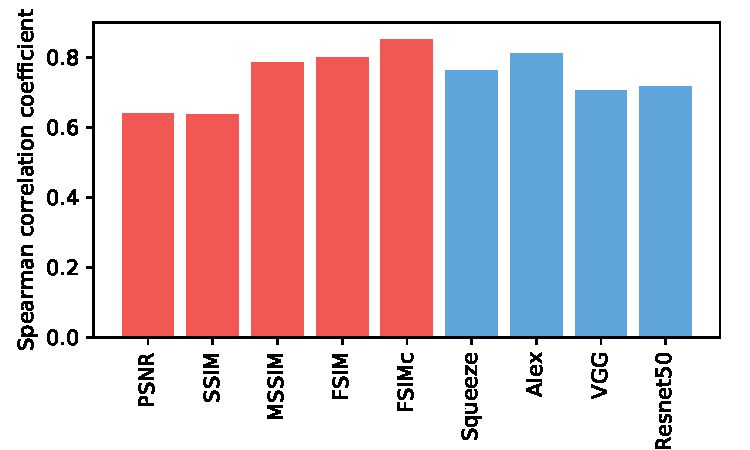
\includegraphics[width=1.\linewidth]{imgs/resultsTID.pdf} \\
\vspace{-2mm}
\caption{\label{fig:tid}
\textbf{TID Dataset} We show the Spearman correlation coefficient of various methods on the TID2013 Dataset~\cite{ponomarenko2015image}. Note that deep networks trained for classification perform well out of the box (blue).
}
\vspace{-3mm}
\end{figure}

\section{TID2013 Dataset}
\label{sec:tid}

In Figure~\ref{fig:tid}, we compute scores on the TID2013~\cite{ponomarenko2015image} dataset. 
We test the images at a different resolutions, using $\{128, 192, 256, 384, 512\}$ for the smaller dimension. 
We note that even averaging across all scales and layers, with no further calibration, the AlexNet~\cite{krizhevsky2014one} architecture gives scores near the highest metric, FSIMc~\cite{zhang2011fsim}. On our traditional perturbations, the FSIMc metric achieves $61.4\%$, close to $\ell_2$ at $59.9\%$, while the deep classification networks we tested achieved $73.3\%$, $70.6\%$, and $70.1\%$, respectively. The difference is likely due to the inclusion of geometric distortions in our dataset. Despite their frequent use in such situations, metrics such as SSIM were not designed to handle geometric distortions~\cite{sampat2009complex}.
